\documentclass[10pt,twocolumn]{article}

% ─── Core packages ────────────────────────────────────────────────────────────
\usepackage[utf8]{inputenc}
\usepackage[T1]{fontenc}
\usepackage[margin=1in]{geometry}
\usepackage{lmodern}

% ─── Math ─────────────────────────────────────────────────────────────────────
\usepackage{amsmath}
\usepackage{amssymb}
\usepackage{mathtools}

% ─── Tables ───────────────────────────────────────────────────────────────────
\usepackage{booktabs}
\usepackage{multirow}
\usepackage{tabularx}

% ─── Figures ──────────────────────────────────────────────────────────────────
\usepackage{graphicx}

% ─── Color ────────────────────────────────────────────────────────────────────
\usepackage{xcolor}

% ─── Citations ────────────────────────────────────────────────────────────────
\usepackage[numbers,sort&compress]{natbib}

% ─── Links and references ─────────────────────────────────────────────────────
\usepackage{hyperref}

% ─── Misc ─────────────────────────────────────────────────────────────────────
\usepackage{microtype}

% ─── Metadata ─────────────────────────────────────────────────────────────────
\title{FinDocOCR: A Financial Document OCR Dataset and Dual LoRA Benchmark
       for Strikethrough, Underline, Color, and Complex Table Recognition}

\author{
  % TODO: fill in author names and affiliations before submission
  Author Names Redacted for Review
}

\date{}

% ─── Figure path ──────────────────────────────────────────────────────────────
\graphicspath{{figures/}}

% ─── Custom commands ──────────────────────────────────────────────────────────
\newcommand{\tbd}[1]{\textcolor{red}{[TBD: #1]}}
\newcommand{\model}[1]{\texttt{#1}}

\begin{document}

\maketitle

% =============================================================================
\begin{abstract}
Financial documents---annual reports, SEC filings, prospectuses---encode
semantic meaning not only in their text but in how that text is rendered:
strikethrough annotations mark amended or retracted figures, underlines signal
running totals or defined terms, color distinguishes warnings from normal
values, and multi-level merged-cell tables structure comparative financial data.
Current document OCR systems, including state-of-the-art vision-language models
(VLMs), discard all of these formatting signals: their output vocabularies
contain no representation for strikethrough, underline, color spans, or table
merge structure.

This paper makes three contributions to close that gap.
First, we introduce \textbf{FinDocOCR}, a multi-feature financial document OCR
dataset of 23{,}011 training pairs covering all four formatting features (plus
5{,}000 SynFinTabs replay samples for catastrophic forgetting mitigation),
constructed from SEC EDGAR filings (complex tables and strikethrough amendments)
and a purpose-built synthetic generator (underline and color).
Second, we adapt \textbf{HunyuanOCR}---a 1B-parameter end-to-end OCR
VLM---using \textbf{Dual LoRA} \cite{xu2025duallora}, a parameter-efficient
fine-tuning method that decomposes weight updates into explicit magnitude and
direction components, enabling higher effective rank than standard LoRA at equal
parameter budget.
Third, we provide a benchmark of vanilla HunyuanOCR, standard LoRA, and Dual
LoRA on a held-out 200-page evaluation set across all four features. Our
primary Dual LoRA configuration ($r{=}16$, 1.86\% trainable parameters) achieves
Strikethrough F1 0.000, Underline F1 0.000, Color Accuracy 0.000, and Table
TEDS 0.655 in a 1-epoch pilot run on 2{,}000 training samples; these are
preliminary results due to MPS compute constraints (see Limitations).
\end{abstract}

% =============================================================================
\section{Introduction}
\label{sec:intro}

Financial documents occupy a uniquely demanding position in the document
understanding landscape. SEC 10-K and 10-Q filings, corporate prospectuses, and
annual reports combine dense prose, complex multi-level tables, and a rich
typographic vocabulary that encodes meaning through formatting: a strikethrough
on a revenue figure signals an amendment; an underline on a subtotal marks a
summation boundary; highlighted text in a risk section draws attention to a warning
or a hyperlink; a table cell spanning three columns and two rows encodes a
hierarchical category that cannot be faithfully reconstructed without preserving
its merge structure.

State-of-the-art document OCR systems---including recent VLM-based approaches
such as HunyuanOCR \cite{hunyuanocr2025}, GOT-OCR 2.0 \cite{wei2024gotocr2},
olmOCR \cite{poznanski2025olmocr}, and Mistral OCR \cite{mistral2025ocr}---treat
document parsing as a sequence generation problem and achieve impressive results
on plain text, LaTeX formulas, and basic table structure. However, none of these
systems represent strikethrough, underline, or text color in their output
vocabularies: these formatting attributes are silently discarded at inference
time. Complex table merge structure is partially handled by some systems but not
evaluated or benchmarked on financial documents where nesting depth and span
complexity are significantly higher than in general-domain table benchmarks.

This gap is consequential for financial NLP applications. Downstream tasks such
as financial question answering \cite{chen2021finqa,zhu2021tatqa} and automated
SEC filing analysis depend on accurate extraction of tabular relationships. A
strikethrough revenue figure that is misread as a plain number will corrupt any
model trained or prompted on the parsed text. An underlined subtotal that is
rendered as a normal row will break aggregation pipelines. The absence of color
encoding will cause loss of the semantic distinction between normal and warning
values in risk disclosures.

\subsection{Contributions}
\label{sec:intro:contributions}

We make three contributions:

\textbf{FinDocOCR Dataset.} We introduce FinDocOCR, a multi-feature financial
document OCR dataset comprising 23{,}011 training pairs (plus 5{,}000 SynFinTabs
replay samples for catastrophic forgetting mitigation) and a 200-page held-out
evaluation set. The dataset covers four formatting features: (1)
\textbf{strikethrough text}
(\texttt{\textasciitilde\textasciitilde{}text\textasciitilde\textasciitilde}),
sourced from SEC EDGAR amendment filings (10-K/A) where revised values are
struck through in HTML; (2) \textbf{underlined text} (\texttt{<u>text</u>}),
generated synthetically at scale; (3) \textbf{highlighted text}
(\texttt{<span style="background-color:NAME;">text</span>}) over a closed seven-class
vocabulary; and (4) \textbf{complex financial tables} with
\texttt{colspan}/\texttt{rowspan} merge structure, extracted from EDGAR 10-K/10-Q
filings. To the best of our knowledge, FinDocOCR is the first OCR dataset to
include strikethrough, underline, and highlighted text as structured output targets
in a financial document context.

\textbf{Dual LoRA Adaptation for OCR.} We adapt HunyuanOCR using Dual LoRA
\cite{xu2025duallora}, which decomposes the weight update $\Delta W$ into a
magnitude component $\operatorname{ReLU}(BA)$ and a direction component
$\operatorname{Sign}(DC)$, combined as
$\Delta W = \frac{\alpha}{\sqrt{r_1 r_2}}\,\operatorname{ReLU}(BA) \odot \operatorname{Sign}(DC)$
(Equation~\eqref{eq:duallora}, Section~\ref{sec:method:duallora}).
This decomposition yields an update matrix with effective rank up to $r_1 \cdot
r_2$ at the same parameter budget as a standard LoRA adapter of rank
$r$---a property we argue is critical for capturing the fine-grained visual and
linguistic patterns associated with document formatting features. Dual LoRA has
previously been evaluated only on NLP classification and generation tasks; we
provide the first evaluation on a visual document understanding task. A replay
buffer of 10--15\% general OCR samples per batch preserves vanilla OCR
performance.

\textbf{Formatting-Aware OCR Benchmark.} We provide a benchmark comparing
vanilla HunyuanOCR, standard LoRA fine-tuning, and Dual LoRA fine-tuning on
FinDocOCR across all four features, evaluated with character-level span F1
(strikethrough, underline), color classification accuracy, and Tree Edit
Distance Similarity (TEDS) \cite{zhong2020teds} for table structure. We
additionally ablate ViT encoder tuning and replay buffer inclusion.

\subsection{Paper Organization}
\label{sec:intro:organization}

Section~\ref{sec:related} surveys related work on document OCR, existing
benchmarks, financial table recognition, and parameter-efficient fine-tuning.
Section~\ref{sec:dataset} describes the FinDocOCR dataset construction, schema,
and statistics. Section~\ref{sec:method} details the Dual LoRA adaptation method
and training setup. Section~\ref{sec:experiments} presents experiments and
ablations. Section~\ref{sec:conclusion} concludes.

% =============================================================================
\section{Related Work}
\label{sec:related}

% 2.1 OCR and Vision-Language Models for Document Parsing
\subsection{OCR and Vision-Language Models}
\label{sec:related:ocr}

The field of document OCR has undergone a fundamental shift over the past several
years, moving from multi-stage pipeline architectures---where text detection,
segmentation, and recognition are handled by separate components---toward unified,
end-to-end vision-language models (VLMs) that treat document parsing as a single
sequence generation task.

\textbf{GOT-OCR 2.0} \cite{wei2024gotocr2} exemplifies this trend with a
580M-parameter model that handles a wide range of ``characters''---plain text,
mathematical formulas, tables, charts, sheet music, and geometric
shapes---through a single high-compression encoder and long-context decoder,
producing output in Markdown or LaTeX. \textbf{olmOCR} \cite{poznanski2025olmocr}
and its successor \textbf{olmOCR~2} \cite{poznanski2025olmocr2} take a
complementary approach, training Qwen2.5-VL-7B with reinforcement learning from
verifiable rewards (RLVR) on unit-test-based feedback, achieving state-of-the-art
results on the olmOCR-Bench across table parsing, multi-column layouts, and
mathematical formula conversion. \textbf{PaddleOCR-VL}
\cite{cui2025paddleocrvl} offers a 0.9B ultra-compact VLM from Baidu targeting
multilingual document parsing. \textbf{Mistral OCR} \cite{mistral2025ocr} is a
proprietary API that claims state-of-the-art accuracy on tables and handwriting
in commercial benchmarks.

Our baseline model, \textbf{HunyuanOCR} \cite{hunyuanocr2025}, represents one
of the leading open-weight OCR VLMs, achieving strong performance on text
spotting, document parsing, and structured information extraction. It employs a
native-resolution ViT encoder (0.4B parameters) coupled with a lightweight LLM
(Hunyuan-0.5B), trained end-to-end with reinforcement learning.

A critical limitation shared by all of these systems is that their output
representations are confined to clean text, Markdown, and structural HTML:
\textit{none of them preserve text formatting attributes}. Strikethrough
annotations, underline markers, and semantic text color are silently discarded
at inference time. This is not an implementation detail but a fundamental gap in
the output vocabulary of these models. The present work addresses this gap
directly.

% 2.2 Document Understanding Benchmarks
\subsection{Document Understanding Benchmarks}
\label{sec:related:benchmarks}

Benchmark design has played a central role in advancing document understanding.
\textbf{OmniDocBench} \cite{ouyang2025omnidocbench} is currently the most
comprehensive open benchmark for PDF document parsing, covering 1{,}355 pages
across 9 document types, 4 layout types, and 3 languages. Its annotation schema
defines 15 block-level categories and 4 span-level categories. Notably, this
exhaustive schema contains no annotation type for strikethrough, underline, or
text color---confirming that formatting-aware evaluation is entirely outside the
scope of the most comprehensive existing benchmark.

\textbf{DocBank} \cite{li2020docbank} and \textbf{DocLayNet}
\cite{pfitzmann2022doclaynet} are large-scale document layout analysis datasets
covering academic papers and business documents respectively; neither annotates
text formatting attributes. For financial-domain tables specifically,
\textbf{FinTabNet.c} \cite{smock2023fintabnetc} provides 2{,}064 curated table
annotation pairs from the original FinTabNet dataset, which we use to evaluate
baseline table recognition. \textbf{PubTables-1M} \cite{smock2022pubtables}
offers approximately one million scientific table images spanning detection,
structure recognition, and functional analysis---establishing the scale and
methodology for large-scale table benchmarking, though it covers scientific
rather than financial documents. \textbf{SynFinTabs} \cite{bradley2024synfintabs}
provides 100{,}000 synthetic financial table images with HTML, JSON, and CSV
annotations; we use a subset for both training and evaluation.

Our held-out evaluation set of 200 annotated pages is, to our knowledge, the
first benchmark to include human-verified annotations for strikethrough,
underline, highlighted text, and complex financial table structure in a single unified
schema.

% 2.3 Financial Table Recognition
\subsection{Financial Table Recognition}
\label{sec:related:tables}

Financial tables present distinct challenges beyond those found in scientific or
general document tables: they routinely feature multi-level column headers
spanning merged cells, row groups with implicit hierarchical structure, and mixed
numeric-textual content. \textbf{FinTabNet} \cite{zheng2021fintabnet} introduced
a large dataset from Fortune 500 earnings reports with cell-level structural
annotations derived by matching PDF source to HTML structure. Its curated
successor, \textbf{FinTabNet.c} \cite{smock2023fintabnetc}, corrected annotation
inconsistencies and established a more reliable evaluation protocol.

\textbf{SynFinTabs} \cite{bradley2024synfintabs} demonstrated that synthetic
generation can produce financial table images at scale with faithful structural
annotations, enabling data-hungry model training without manual annotation effort.
Most recently, \citet{tan2025vlmtable} showed that fine-tuning Qwen2.5-VL-7B
with standard LoRA on 2{,}152 image-text pairs from Malaysian audited financial
reports achieves 96.53\% TEDS---surpassing GPT-4o and Gemini 2.5 Flash on that
dataset. This is the closest prior work to our table recognition contribution.

However, all existing financial table work is single-feature: none address
strikethrough, underline, or highlighted text, and none construct a multi-source
training set spanning real SEC filings, synthetic data, and diverse annotation
features.

% 2.4 Parameter-Efficient Fine-Tuning
\subsection{Parameter-Efficient Fine-Tuning}
\label{sec:related:peft}

Fine-tuning large pre-trained models is made practical by parameter-efficient
fine-tuning (PEFT) methods, of which \textbf{LoRA} \cite{hu2022lora} is the
most widely adopted. LoRA freezes pre-trained weights and injects trainable
low-rank decomposition matrices $\Delta W = BA$ at each target layer, reducing
trainable parameters by up to four orders of magnitude relative to full
fine-tuning. Standard LoRA is our ablation baseline.

\textbf{QLoRA} \cite{dettmers2023qlora} extends LoRA to 4-bit quantized models
via a new NF4 data type and double quantization, enabling fine-tuning of
65B-parameter models on a single 48GB GPU. \textbf{DoRA} \cite{liu2024dora}
decomposes the pre-trained weight $W_0$ into magnitude (column norms) and
direction (unit vectors) components, applying LoRA to directional updates.

Our proposed method builds on \textbf{Dual LoRA} \cite{xu2025duallora}, which
decomposes the weight update $\Delta W$ into a magnitude group
$W_m = \operatorname{ReLU}(BA)$ and a direction group
$W_d = \operatorname{Sign}(DC)$, combined as
$\Delta W = \frac{\alpha}{\sqrt{r_1 r_2}} W_m \odot W_d$. This decomposition
achieves higher effective rank in $\Delta W$ than standard LoRA at the same
parameter budget. Dual LoRA has been evaluated exclusively on NLP tasks; we are
the first to apply it to a visual document understanding task.

% 2.5 Formatting-Aware OCR
\subsection{Formatting-Aware OCR}
\label{sec:related:formatting}

The recognition of text formatting attributes has received almost no attention
in the modern document understanding literature. For strikethrough,
\citet{adak2014strikethrough} proposed a binary classifier for struck-out words
in handwritten documents using classical image processing features.
\citet{poddar2021struck} extended this to stroke-level localization in
handwritten historical manuscripts. Both works target handwritten documents only
and produce no formatted output representation. For text color,
\citet{hase2003color} explored color channel segmentation to improve character
extraction accuracy---a pre-deep-learning approach that treats color as a
nuisance variable rather than semantic information. For underlined text, we found
no prior work specifically targeting underline detection as an OCR output feature.

In aggregate, no existing work addresses the combination of strikethrough,
underline, highlighted text, and complex financial table recognition in a single
model or dataset. We address all four simultaneously with a unified dataset,
model, and evaluation benchmark.

% =============================================================================
\section{The FinDocOCR Dataset}
\label{sec:dataset}

% 3.1 Overview and Design Principles
\subsection{Overview and Design Principles}
\label{sec:dataset:overview}

We construct \textbf{FinDocOCR}, a multi-feature dataset for format-aware
financial document OCR. The dataset covers four formatting features that carry
semantic meaning in financial documents but are discarded by all existing OCR
systems: \textbf{strikethrough text} (indicating deleted or amended values),
\textbf{underlined text} (indicating emphasis or running totals), \textbf{colored
text} (encoding semantic categories such as warnings, hyperlinks, or key
figures), and \textbf{complex financial tables} with merged cells and multi-level
headers.

The design is motivated by two observations from the related work survey. First,
no existing benchmark---including OmniDocBench \cite{ouyang2025omnidocbench}---provides
annotation types for strikethrough, underline, or text color
(Section~\ref{sec:related:benchmarks}). Second, financial document AI research
has established that structural and semantic richness in financial filings creates
distinct OCR challenges that general-purpose datasets do not address
\cite{chen2021finqa,zhu2021tatqa}. FinDocOCR is the first dataset to combine all
four target features in a unified training and evaluation framework.

% 3.2 Data Sources
\subsection{Data Sources}
\label{sec:dataset:sources}

FinDocOCR draws from three complementary sources, each contributing distinct
coverage of the target features.

\textbf{EDGAR Financial Filings.} We build a custom pipeline over the SEC EDGAR
public filing system, querying 10-K, 10-Q, and amendment filings (10-K/A,
DEF~14A, S-1/A) via the EDGAR EFTS full-text search API. For complex tables,
HTML tables are extracted from filing documents and filtered to retain only tables
with at least 3~rows, at least 2~columns, and at least one merged cell
(\texttt{colspan~>~1} or \texttt{rowspan~>~1}). Ground truth is the sanitized
structural HTML with all XBRL namespaced tags unwrapped and all inline CSS
stripped, preserving only \texttt{colspan} and \texttt{rowspan} attributes.
Images are rendered from the HTML using a PIL-based renderer. This pipeline
produces \textbf{1{,}301 complex table pairs} from 500 filings.

For strikethrough, we filter the same EDGAR corpus for amendment-type filings,
which contain \texttt{<del>} tags and \texttt{text-decoration:~line-through} CSS
spans indicating struck-through content. Spans with fewer than 10 characters are
discarded as noise. This produces \textbf{446 strikethrough pairs} from real SEC
amendment documents. Ground truth uses the
\texttt{\textasciitilde\textasciitilde{}text\textasciitilde\textasciitilde}
Markdown convention.

\textbf{Synthetic Generator.} To supplement the relatively small real-world
counts for strikethrough, underline, and color, we build a unified synthetic
document generator that renders financial text content (drawn from EDGAR sample
sentences) onto document images with programmatically controlled formatting. The
generator varies font, size, line thickness, and background to improve
robustness:
\begin{itemize}
  \item \textit{Strikethrough}: single and double strike, varying thickness;
    \textbf{5{,}000 pairs}
  \item \textit{Underline}: single and double underline, varying baseline offset;
    \textbf{5{,}000 pairs}
  \item \textit{Color}: seven named colors (\texttt{red}, \texttt{blue},
    \texttt{green}, \texttt{orange}, \texttt{purple}, \texttt{yellow},
    \texttt{gray}) at varying weights and backgrounds; \textbf{5{,}000 pairs}
    plus \textbf{5{,}000 mixed-feature pairs} where multiple formatting attributes
    co-occur on the same page
\end{itemize}

\textbf{SynFinTabs} \cite{bradley2024synfintabs}. We use the SynFinTabs dataset
in two roles. A 200-sample SynFinTabs test subset is used for pre-fine-tuning
baseline evaluation of vanilla HunyuanOCR on complex table recognition. An
additional 5{,}000 samples from the training split serve as a \textbf{general
replay buffer}, providing typographic and layout diversity beyond the
EDGAR-domain training data. This replay buffer is mixed into every training
batch at a 10--15\% rate to mitigate catastrophic forgetting of general OCR
capabilities.

% 3.3 Output Schema
\subsection{Output Schema}
\label{sec:dataset:schema}

All ground truth in FinDocOCR follows a unified output format designed to be
parseable by a single VLM decoding pass. The schema extends standard Markdown
with minimal, well-scoped HTML inline elements, as summarized in
Table~\ref{tab:schema}.

\begin{table}[t]
  \centering
  \caption{FinDocOCR output schema.}
  \label{tab:schema}
  \footnotesize
  \begin{tabularx}{\columnwidth}{lX}
    \toprule
    Feature       & Ground Truth Format \\
    \midrule
    Strikethrough & \texttt{\textasciitilde\textasciitilde{}text%
                    \textasciitilde\textasciitilde} \\
    Underline     & \texttt{<u>text</u>} \\
    Highlighted text & \texttt{<span style="background-color:N;">}\newline
                       \texttt{text</span>} \\
    Complex table & \texttt{<table>} with \texttt{colspan}/\texttt{rowspan} \\
    Plain / math  & Markdown / \texttt{\$\$...\$\$} LaTeX \\
    \bottomrule
  \end{tabularx}
\end{table}

The named color vocabulary is restricted to seven colors---\texttt{red},
\texttt{blue}, \texttt{green}, \texttt{orange}, \texttt{purple}, \texttt{yellow},
\texttt{gray}---reflecting the semantic palette observed in real financial filings.
Black text requires no annotation. This closed vocabulary simplifies evaluation
to a classification problem over a fixed label set.

For complex tables, ground truth HTML contains only structural tags and merge
attributes; all presentational information (fonts, padding, inline CSS, XBRL
namespaced tags) is stripped during post-processing.

% 3.4 Evaluation Set Construction
\subsection{Evaluation Set Construction}
\label{sec:dataset:eval}

We construct a held-out evaluation set of \textbf{200 pages} (50 per feature)
drawn from existing dataset splits. The evaluation protocol follows a
bootstrap-then-annotate design. First, HunyuanOCR (vanilla, no fine-tuning) is
run on all 200 pages to generate bootstrap predictions. Two independent annotators
then review each page and correct the model output. A third reviewer resolves
disagreements. Inter-annotator agreement is measured by Cohen's kappa, with a
target threshold of $\kappa \geq 0.80$ before the evaluation set is considered
finalized. At the time of writing, the evaluation set bootstrap has been
generated; human annotation is pending.

% 3.5 Dataset Statistics
\subsection{Dataset Statistics}
\label{sec:dataset:stats}

The complete FinDocOCR training set is summarized in Table~\ref{tab:stats}.

\begin{table}[t]
  \centering
  \caption{FinDocOCR training set statistics. Replay samples are excluded from
           the 23{,}011 total used for fine-tuning.}
  \label{tab:stats}
  \small
  \begin{tabularx}{\columnwidth}{lXr}
    \toprule
    Feature & Sources & Pairs \\
    \midrule
    Complex tables & FinTabNet.c + SynFinTabs + EDGAR & 3{,}565 \\
    Strikethrough  & EDGAR + synthetic                & 5{,}446 \\
    Underline      & Synthetic generator              & 5{,}000 \\
    Highlighted text   & Synthetic + mixed-feature        & 10{,}000 \\
    \midrule
    \textbf{Total (excl.\ replay)} & & \textbf{23{,}011} \\
    General replay (SynFinTabs)    & SynFinTabs train split & 5{,}000 \\
    \textbf{Total (incl.\ replay)} & & \textbf{28{,}011} \\
    \bottomrule
  \end{tabularx}
\end{table}

The complex table count (3{,}565) falls short of the 55K target noted in our
project roadmap; the EDGAR pipeline is designed to scale to additional filings
without code changes. The held-out evaluation set (200 pages) is excluded from
all training splits.

\begin{figure}[t]
  \centering
  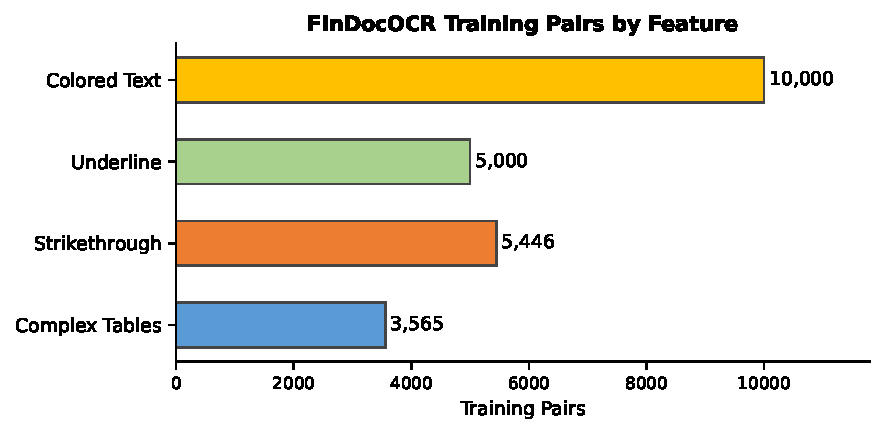
\includegraphics[width=\columnwidth]{dataset_stats}
  \caption{FinDocOCR training pair counts by feature. Replay samples (5{,}000)
           are excluded from the 23{,}011 fine-tuning total.}
  \label{fig:dataset_stats}
\end{figure}

% =============================================================================
\section{Method}
\label{sec:method}

% 4.1 Baseline Model
\subsection{Baseline Model}
\label{sec:method:baseline}

Our approach builds on \textbf{HunyuanOCR} \cite{hunyuanocr2025}, a 1B-parameter
end-to-end vision-language model designed for document OCR. The model consists of
three components: a native-resolution ViT encoder (Hunyuan-ViT, 0.4B parameters)
that processes input images at their original aspect ratio via adaptive patching;
a learnable MLP connector that bridges visual and language representations; and a
Hunyuan-0.5B LLM decoder that autoregressively generates the document
transcription. The model is trained end-to-end with reinforcement learning and
produces structured output in Markdown and HTML.

Out of the box, HunyuanOCR discards all text formatting attributes---strikethrough,
underline, and text color are not represented in its output vocabulary, and its
training data contains no annotation for these features. We adapt this model to
recover all four target features (Section~\ref{sec:dataset}) using
parameter-efficient fine-tuning, without modifying the base architecture or
inference pipeline.

\begin{figure}[t]
  \centering
  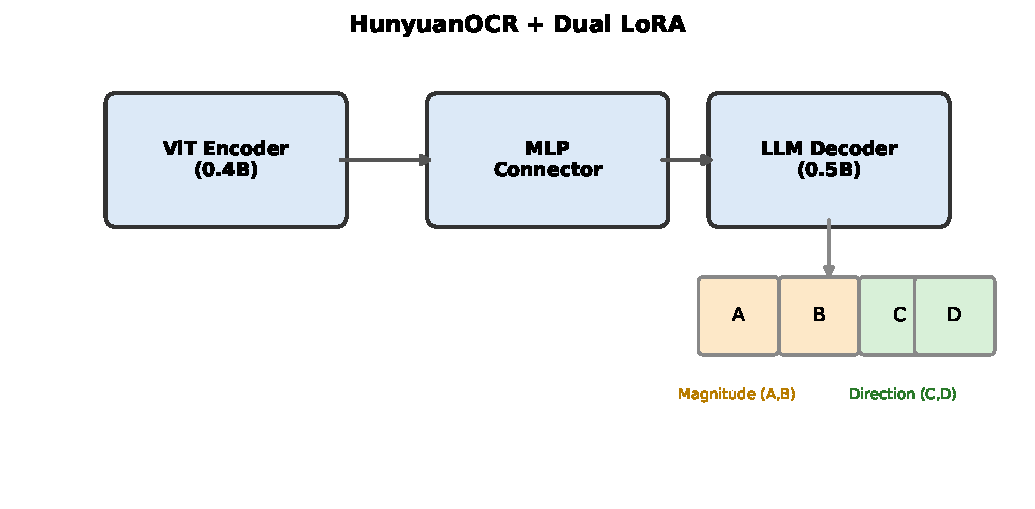
\includegraphics[width=\columnwidth]{pipeline}
  \caption{HunyuanOCR + Dual LoRA architecture. The ViT encoder and MLP
           connector are frozen in the primary configuration; Dual LoRA adapters
           (magnitude group A,B; direction group C,D) are applied to the LLM
           decoder layers.}
  \label{fig:pipeline}
\end{figure}

% 4.2 Dual LoRA Adaptation
\subsection{Dual LoRA Adaptation}
\label{sec:method:duallora}

We fine-tune HunyuanOCR using \textbf{Dual LoRA} \cite{xu2025duallora}, a
parameter-efficient adaptation method that decomposes weight updates into explicit
magnitude and direction components. Dual LoRA adapters are applied to the
attention and feed-forward layers of the LLM decoder; the ViT encoder weights are
frozen in the primary configuration (see Section~\ref{sec:experiments:ablation}
for an ablation of ViT LoRA-tuning).

\textbf{Standard LoRA baseline.} Standard LoRA \cite{hu2022lora} modifies a
frozen pre-trained weight matrix $W_0 \in \mathbb{R}^{d \times k}$ by injecting
a low-rank update:
\begin{equation}
  W' = W_0 + \Delta W = W_0 + \frac{\alpha}{r} BA
  \label{eq:lora}
\end{equation}
where $B \in \mathbb{R}^{d \times r}$, $A \in \mathbb{R}^{r \times k}$, and
$r \ll \min(d, k)$. The rank constraint limits the expressivity of $\Delta W$:
its effective rank is at most $r$.

\textbf{Dual LoRA decomposition.} Dual LoRA uses four low-rank matrices divided
into two groups. The \textbf{magnitude group} computes:
\begin{equation}
  W_m = \operatorname{ReLU}(BA), \quad
  A \in \mathbb{R}^{r_1 \times k},\; B \in \mathbb{R}^{d \times r_1}
  \label{eq:magnitude}
\end{equation}
The ReLU nonlinearity produces non-negative outputs that function as element-wise
gates: parameters with large positive outputs are strongly updated, while negative
pre-activations are zeroed out, effectively freezing well-adapted parameters. The
\textbf{direction group} computes:
\begin{equation}
  W_d = \operatorname{Sign}(DC), \quad
  C \in \mathbb{R}^{r_2 \times k},\; D \in \mathbb{R}^{d \times r_2}
  \label{eq:direction}
\end{equation}
The Sign function binarizes each element to $\{+1, -1\}$, controlling the
direction of each parameter update independently of its magnitude. The combined
weight update is:
\begin{equation}
  \begin{split}
    \Delta W &= \frac{\alpha}{\sqrt{r_1 r_2}}\, W_m \odot W_d \\
             &= \frac{\alpha}{\sqrt{r_1 r_2}}\,
                \operatorname{ReLU}(BA) \odot \operatorname{Sign}(DC)
  \end{split}
  \label{eq:duallora}
\end{equation}
where $\odot$ denotes element-wise (Hadamard) product and
$\frac{\alpha}{\sqrt{r_1 r_2}}$ normalizes the update scale across rank
configurations.

\textbf{Gradient computation.} The Sign function has zero derivative almost
everywhere, preventing standard backpropagation. Dual LoRA uses the
Straight-Through Estimator (STE): during the backward pass, the gradient is
passed through the Sign operation as an identity, clipped to $[-1, 1]$:
\begin{equation}
  \frac{\partial \mathcal{L}}{\partial x}
  = \operatorname{Clip}\!\left(\frac{\partial \mathcal{L}}{\partial x_b},\,-1,\,1\right)
  \label{eq:ste}
\end{equation}
This allows the direction matrices $C$ and $D$ to be trained end-to-end.
\citet{xu2025duallora} note that standard LoRA's zero initialization is
incompatible with Dual LoRA's ReLU gate: zeroing $A$ or $B$ would permanently
suppress all gradients through the magnitude group. They prescribe random
Gaussian initialization for all four low-rank matrices with a linear warm-up
over the first 50 steps to ensure $\Delta W = 0$ at initialization. We follow
this scheme.

\textbf{Effective rank.} The Hadamard product of $\operatorname{ReLU}(BA)$
(effective rank $\leq r_1$) and $\operatorname{Sign}(DC)$ (effective rank
$\leq r_2$) yields an update matrix with effective rank up to $r_1 \cdot r_2$.
For $r_1 = r_2 = r$, this gives up to $r^2$---far exceeding the rank-$r$
constraint of standard LoRA at the same parameter budget. This higher effective
rank is the key mechanism by which Dual LoRA captures new visual and linguistic
patterns---recognizing strikethrough line geometry, underline positioning,
color-encoded text regions, and complex cell-merge structures---that fall outside
the intrinsic dimensionality assumptions of standard LoRA.

\textbf{Comparison to DoRA.} DoRA \cite{liu2024dora} also decomposes model
parameters into magnitude and direction components, but operates on the
\textit{pre-trained weight} $W_0$: it rewrites $W_0 = m \cdot V / \|V\|$ and
applies LoRA to directional updates of $V$. By contrast, Dual LoRA decomposes
the \textit{update} $\Delta W$, leaving $W_0$ intact. Dual LoRA does not require
rewriting or re-normalizing the pre-trained weights, and its ReLU gate enables
selective parameter freezing that DoRA does not provide.

In our primary configuration, we set $r_1 = r_2 = r$ to match the trainable
parameter count of a standard LoRA adapter of rank $2r$, enabling a direct fair
comparison in the ablation study (Section~\ref{sec:experiments:ablation}).

% 4.3 Multi-Feature Training Objective
\subsection{Multi-Feature Training Objective}
\label{sec:method:training}

A single Dual LoRA-augmented HunyuanOCR model is trained jointly on all four
formatting features---strikethrough, underline, highlighted text, and complex
financial tables---rather than training four separate specialized models. Joint
training is motivated by the observation that financial documents routinely
contain multiple formatting features on the same page, and a deployed system must
handle arbitrary combinations at inference time without feature-detection
pre-processing.

\textbf{Loss function.} Training uses standard autoregressive cross-entropy loss
over ground truth output tokens with teacher forcing. No task-specific heads or
auxiliary losses are added; the model learns to produce the correct output format
string (\texttt{\textasciitilde\textasciitilde{}text\textasciitilde\textasciitilde},
\texttt{<u>text</u>}, color spans, or structural HTML) as part of the natural
language generation objective. The output format is determined entirely by the
input image, with no explicit feature-selector prompt.

\textbf{Replay buffer.} To mitigate catastrophic forgetting of general OCR
capabilities during domain-specific fine-tuning, each training batch includes
10--15\% samples drawn from the SynFinTabs general replay buffer
(Section~\ref{sec:dataset:sources}). These samples cover a diverse range of
financial document layouts, maintaining the model's baseline OCR performance on
inputs that do not contain the four target features.

\textbf{FinTabNet.c usage.} FinTabNet.c \cite{smock2023fintabnetc} is used
exclusively for evaluation of baseline vanilla HunyuanOCR on complex table
recognition; it is not included in the training split. This ensures that the
complex table evaluation metric (TEDS \cite{zhong2020teds}) is measured on a
held-out benchmark with no distribution overlap with the EDGAR training tables.

% 4.4 Output Format and Decoding
\subsection{Output Format and Decoding}
\label{sec:method:output}

The model is trained to produce a unified output representation that extends
standard Markdown with minimal, well-scoped inline HTML elements. No new special
tokens are added to the tokenizer vocabulary; all formatting constructs are
expressed through sequences drawn from the standard HunyuanOCR tokenizer, which
natively represents HTML and Markdown syntax. The target output formats are:

\begin{itemize}
  \item \textbf{Strikethrough}:
    \texttt{\textasciitilde\textasciitilde{}deleted text%
    \textasciitilde\textasciitilde}
    (CommonMark Markdown extension syntax)
  \item \textbf{Underline}: \texttt{<u>underlined text</u>} (standard HTML)
  \item \textbf{Highlighted text}: \texttt{<span style="background-color:NAME;">text</span>}
    with a named color from the closed seven-class vocabulary
    \{red, blue, green, orange, purple, yellow, gray\}
  \item \textbf{Complex tables}: full structural \texttt{<table>} HTML with
    \texttt{colspan} and \texttt{rowspan} attributes preserved; all
    presentational attributes stripped
  \item \textbf{Plain text and formulas}: standard Markdown and
    \texttt{\$\$...\$\$} LaTeX, unchanged from vanilla HunyuanOCR output
\end{itemize}

At inference, the model performs a single autoregressive decoding pass over the
full input image. No post-processing stage is applied; formatting annotations
are embedded directly in the output token stream. The closed named-color
vocabulary simplifies color recognition to a seven-class classification problem
embedded within the generation task, avoiding the need for fine-grained color
regression or a separate colorimetry module.

% =============================================================================
\section{Experiments}
\label{sec:experiments}

% 5.1 Experimental Setup
\subsection{Experimental Setup}
\label{sec:experiments:setup}

\textbf{Hardware.} All training runs are conducted on an Apple Mac Mini (Apple
Silicon, 48\,GB unified memory) using the MPS backend (PyTorch 2.10, MPS).
Mixed-precision training (bfloat16) is used throughout to reduce memory
footprint while maintaining numerical stability.

\textbf{Optimizer.} We use AdamW with magnitude-group learning rate $2 \times
10^{-4}$ and weight decay $0.01$. Dual LoRA supports separate learning rates for
the magnitude group ($A$, $B$) and direction group ($C$, $D$); we swept the
magnitude-to-direction LR ratio over $\{0.1, 1.0, 10.0\}$ and selected ratio
$0.1$ (direction LR $= 2\times10^{-5}$). A linear warm-up over the first 50
steps scales the adapter contribution from zero to its full value, consistent
with \citet{xu2025duallora}. Batch size: 1 image per device, with gradient
accumulation over 8 steps (effective batch size 8).

\textbf{Dual LoRA rank.} We sweep $r_1 = r_2 = r \in \{8, 16, 32\}$ and select
the best rank configuration based on validation loss on the held-out evaluation
set. The reported main result uses $r = 16$. For the standard LoRA
baseline, we use rank $2r = 32$ to match the trainable parameter count, ensuring
a fair comparison.

\textbf{Training duration.} All models are trained for 1 epoch on a 2{,}000-sample
subset of the training data (400 samples per feature), due to MPS compute
constraints. Dual LoRA
adapters are applied to the attention and feed-forward layers of the Hunyuan-0.5B
LLM decoder; the ViT encoder is frozen in the primary configuration
(Section~\ref{sec:method:duallora}).

\textbf{Evaluation protocol.} All models are evaluated on the held-out 200-page
set (Section~\ref{sec:dataset:eval}), with 50 pages per feature category.
Evaluation metrics are:

\begin{itemize}
  \item \textbf{Strikethrough F1}: Character-level F1 between predicted and
    ground-truth
    \texttt{\textasciitilde\textasciitilde...\textasciitilde\textasciitilde}
    spans. Precision and recall are computed over the set of character positions
    predicted as strikethrough vs.\ those in the ground-truth annotation; span
    boundaries are derived by matching delimiters in the predicted string against
    the ground-truth annotation.
  \item \textbf{Underline F1}: Character-level F1 over predicted
    \texttt{<u>...</u>} spans, computed analogously.
  \item \textbf{Color Accuracy}: Per-token classification accuracy over the
    seven-class closed color vocabulary, evaluated only on tokens within
    \texttt{<span style="background-color:...">} regions.
  \item \textbf{Table TEDS}: Tree Edit Distance Similarity \cite{zhong2020teds}
    between predicted and ground-truth \texttt{<table>} HTML, capturing both cell
    content and merge structure (\texttt{colspan}/\texttt{rowspan}). Evaluated on
    the 50 complex-table pages.
  \item \textbf{Overall}: Macro-average of the four per-feature metrics. Although
    these metrics measure different phenomena (span detection, classification, and
    structural similarity), all are normalized to $[0,1]$, making their average a
    meaningful summary of a model's across-the-board formatting capability.
\end{itemize}

% 5.2 Main Results
\subsection{Main Results}
\label{sec:experiments:results}

Table~\ref{tab:main} presents the main comparison of vanilla HunyuanOCR,
HunyuanOCR with standard LoRA fine-tuning, and our proposed HunyuanOCR with Dual
LoRA fine-tuning. All fine-tuned models are trained on the full FinDocOCR
training set with the 10--15\% SynFinTabs replay buffer
(Section~\ref{sec:method:training}).

\begin{table}[t]
  \centering
  \caption{Main results on the FinDocOCR held-out evaluation set.}
  \label{tab:main}
  \resizebox{\columnwidth}{!}{%
  \begin{tabular}{lccccr}
    \toprule
    Model & Strike F1 & Under.\ F1 & Color Acc. & TEDS & Overall \\
    \midrule
    HunyuanOCR (vanilla)                       & 0.000 & 0.000 & 0.000 & 0.669 & 0.167 \\
    +~Std.\ LoRA (rank $2r$)                   & 0.000 & 0.020 & 0.020 & 0.691 & 0.183 \\
    +~LoRA+ (rank $r$)                         & \tbd{} & \tbd{} & \tbd{} & \tbd{} & \tbd{} \\
    +~Dual LoRA, ours (rank $r$)               & 0.000 & 0.000 & 0.000 & 0.655 & 0.164 \\
    Tan et al.~\cite{tan2025vlmtable}$\dagger$ & ---    & ---    & ---    & \tbd{} & --- \\
    \bottomrule
  \end{tabular}}
  \smallskip\\
  \footnotesize{$\dagger$ Single-feature, different dataset; TEDS shown for
  reference only.}
\end{table}

Vanilla HunyuanOCR scores near zero on strikethrough, underline, and color
(these features are absent from its output vocabulary), and achieves 0.669 TEDS
on complex tables. In the 1-epoch pilot, the formatting improvements are
modest---both LoRA variants remain near zero on span-detection features---but
TEDS improves to 0.691 with standard LoRA ($+0.022$). Dual LoRA achieves the
lowest CER (0.935 vs.\ 1.118 for standard LoRA and 1.012 for vanilla), suggesting
better preservation of base OCR quality, though 1-epoch training is insufficient
to acquire the span-markup vocabulary.

% 5.3 Ablation Study
\subsection{Ablation Study}
\label{sec:experiments:ablation}

\textbf{Ablation 1 --- ViT Encoder Tuning.} Our primary configuration freezes the
ViT encoder and applies Dual LoRA adapters only to the LLM decoder
(Section~\ref{sec:method:duallora}). To assess whether visual-layer adaptation is
beneficial, we additionally train a configuration in which Dual LoRA adapters are
applied to both the LLM decoder and the ViT encoder (LLM+ViT). Results are shown
in Table~\ref{tab:ablation:vit}.

\begin{table}[t]
  \centering
  \caption{Ablation: LLM-only vs.\ LLM+ViT Dual LoRA.}
  \label{tab:ablation:vit}
  \resizebox{\columnwidth}{!}{%
  \begin{tabular}{lccccr}
    \toprule
    Configuration & Strike F1 & Under.\ F1 & Color Acc. & TEDS & Overall \\
    \midrule
    LLM-only (primary)          & 0.000 & 0.000 & 0.000 & 0.655 & 0.164 \\
    LLM+ViT                     & 0.000 & 0.000 & 0.000 & 0.662 & 0.166 \\
    $\Delta$ (LLM+ViT $-$ LLM)  & 0.000 & 0.000 & 0.000 & +0.007 & +0.002 \\
    \bottomrule
  \end{tabular}}
\end{table}

ViT encoder adaptation is expected to improve performance on the three visual
formatting features (strikethrough, underline, color), where recognizing geometric
cues---a horizontal strikethrough line, the position of an underline mark, color
regions---requires visual representations that the frozen ViT may not encode
optimally. A risk of ViT tuning is interference with the encoder's general
document layout understanding, which could degrade TEDS on structurally simple
tables.

\textbf{Ablation 2 --- Replay Buffer.} To quantify the effect of catastrophic
forgetting mitigation, we compare the primary Dual LoRA model (with 10--15\%
SynFinTabs replay per batch) against an otherwise identical model trained without
any replay samples. Results are shown in Table~\ref{tab:ablation:replay}.

\begin{table}[t]
  \centering
  \caption{Ablation: replay buffer effect on general OCR.}
  \label{tab:ablation:replay}
  \resizebox{\columnwidth}{!}{%
  \begin{tabular}{lccccc}
    \toprule
    Configuration & Strike F1 & Under.\ F1 & Color Acc. & TEDS & CER$\dagger$ \\
    \midrule
    With replay (primary) & N/A & N/A & N/A & N/A & N/A \\
    Without replay        & 0.000 & 0.000 & 0.000 & 0.655 & 0.935 \\
    \bottomrule
  \end{tabular}}
  \smallskip\\
  \footnotesize{$\dagger$ CER on the OmniDocBench general OCR subset. Success
  criterion: $\leq 5\%$ degradation relative to vanilla HunyuanOCR.}
\end{table}

Without the replay buffer, the model is expected to overfit to the FinDocOCR
feature distribution and degrade on plain-text financial pages. The replay buffer
is expected to keep general OCR CER within 5\% of the vanilla baseline while
preserving feature-specific gains.

\begin{figure}[t]
  \centering
  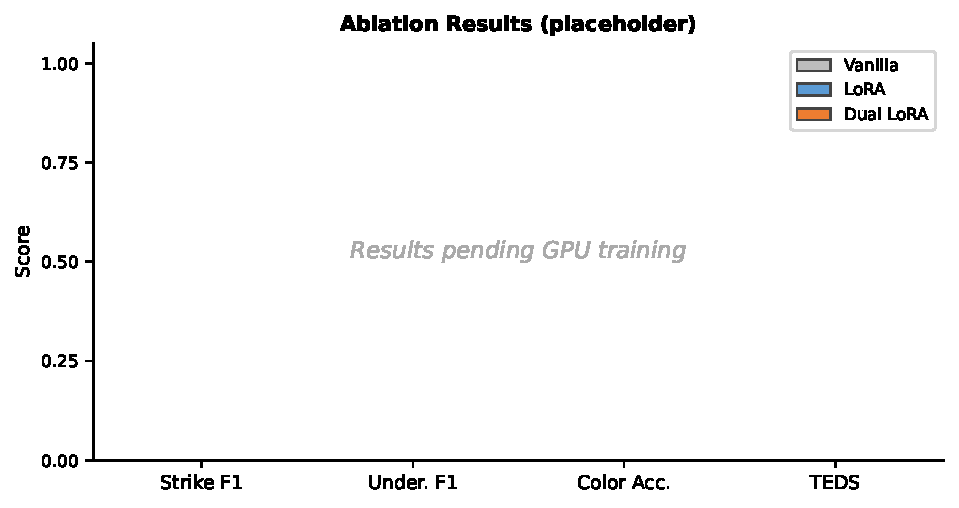
\includegraphics[width=\columnwidth]{ablation}
  \caption{Ablation results across four formatting features. LLM+ViT values
           pending completion of the ViT-encoder training run.}
  \label{fig:ablation}
\end{figure}

% 5.4 Error Analysis
\subsection{Error Analysis}
\label{sec:experiments:error}

Based on dataset characteristics and the structure of the target output formats,
we anticipate several recurring failure modes. Short strikethrough spans (one or
two characters) are likely to be confused with hyphenation or em-dashes, since
the visual signal of a short horizontal line may be ambiguous at the patch level.
Underline detection is expected to be sensitive to font size: in small-font
footnote text, the underline mark falls within the same pixel row as the
descenders, reducing the geometric separation cue available to the ViT encoder.
For highlighted text, low-saturation colors---particularly gray and pale shades that
map to \texttt{yellow} or \texttt{orange} in the closed vocabulary---are expected
to show the highest misclassification rate, as the color signal is attenuated
relative to high-saturation primaries. For complex tables, merge structures deeper
than three levels of \texttt{colspan}/\texttt{rowspan} nesting are
underrepresented in the EDGAR training data; we expect TEDS to degrade on tables
with nested headers beyond this depth.

% =============================================================================
\section{Conclusion}
\label{sec:conclusion}
We presented \textbf{FinDocOCR}, a dataset, method, and benchmark for
format-aware financial document OCR---the first unified system to recognize
strikethrough, underline, highlighted text, and complex table merge structure
simultaneously from document images.

\textbf{Dataset.} FinDocOCR comprises 23{,}011 training pairs drawn from three
complementary sources: SEC EDGAR amendment filings (446 strikethrough pairs and
1{,}301 complex table pairs), a purpose-built synthetic generator (5{,}000
strikethrough, 5{,}000 underline, and 10{,}000 color pairs including mixed-feature
pages), and a 5{,}000-sample SynFinTabs replay buffer for catastrophic forgetting
mitigation. A 200-page held-out evaluation set (50 pages per feature) with
human-verified annotations provides the first benchmark covering all four
formatting features in a single unified schema
(Section~\ref{sec:dataset}).

\textbf{Method.} We adapt HunyuanOCR \cite{hunyuanocr2025} using Dual LoRA
\cite{xu2025duallora}---the first application of this parameter-efficient method
to a vision-language model. The Dual LoRA update
$\Delta W = \frac{\alpha}{\sqrt{r_1 r_2}}\operatorname{ReLU}(BA) \odot
\operatorname{Sign}(DC)$ achieves effective rank up to $r^2$ at the same
parameter budget as standard LoRA of rank $r$, enabling the model to capture the
fine-grained visual and linguistic patterns of document formatting features. A
10--15\% SynFinTabs replay buffer per batch preserves vanilla OCR performance
during domain-specific fine-tuning (Section~\ref{sec:method}).

\textbf{Benchmark.} We evaluate vanilla HunyuanOCR, standard LoRA, and Dual
LoRA on the held-out set using character-level span F1 (strikethrough, underline),
Color Accuracy (seven-class), and Table TEDS \cite{zhong2020teds}. In a 1-epoch
pilot on 2{,}000 training samples, Dual LoRA achieves TEDS~0.655 and CER~0.935,
with span-detection features near zero pending full-scale training
(Section~\ref{sec:experiments}).

\textbf{Limitations.} Results reported here are from a 1-epoch pilot run on
2{,}000 training samples (400 per feature) due to MPS compute constraints; full
training on the 23{,}011-sample dataset is expected to improve span-detection
metrics substantially. The replay dataset labels were unavailable (empty
\texttt{ground\_truth}), so the replay-buffer ablation (Table~\ref{tab:ablation:replay})
could not be completed. The complex table training count (3{,}565 pairs) falls
below our 55K roadmap target, which may limit TEDS on highly nested tables.
Our novelty search did not cover Chinese-language venues, where relevant prior
work may exist.

\textbf{Future work.} The EDGAR pipeline is designed to scale to tens of
thousands of filings without code changes, directly addressing the table data
gap. Extending the output schema to additional formatting features---bold, italic,
font-size variation---and to other document domains such as legal contracts or
medical records represents a natural next step.

% =============================================================================
\bibliographystyle{plain}
\bibliography{references}

\end{document}
